\documentclass[UTF8,a4paper,zihao=-4,fontset=mac]{ctexart}

\usepackage[left=2.55cm,right=2.55cm,top=2.55cm,bottom=2.45cm]{geometry}
\usepackage{graphicx}
\usepackage{booktabs}
\usepackage{tabularx}
\usepackage{longtable}
\usepackage{array}
\usepackage[table]{xcolor}
\usepackage{setspace}
\usepackage{enumitem}
\usepackage{float}
\usepackage{caption}
\usepackage{subcaption}
\usepackage{fancyhdr}
\usepackage{titlesec}
\usepackage{tikz}
\usetikzlibrary{arrows.meta,positioning,calc,shapes.geometric}
\usepackage{pifont}
\usepackage{hyperref}
\usepackage{bookmark}

\definecolor{PetGreen}{HTML}{174A3A}
\definecolor{PetGreenTwo}{HTML}{2E6A55}
\definecolor{PetOrange}{HTML}{D46D4C}
\definecolor{PetCream}{HTML}{F7F2E8}
\definecolor{PetPale}{HTML}{EAF2EE}
\definecolor{PetGray}{HTML}{65706B}
\definecolor{RuleGray}{HTML}{D6DED9}
\definecolor{PetGold}{HTML}{B78A3B}

\hypersetup{
  colorlinks=true,
  linkcolor=PetGreen,
  urlcolor=PetGreenTwo,
  citecolor=PetGreen,
  bookmarksnumbered=true,
  bookmarksopen=true,
  pdfauthor={琚昊，韩旭},
  pdftitle={PetLink 第三阶段第2周开发进展报告},
  pdfsubject={软件课程设计 I 阶段进展报告}
}

\setstretch{1.5}
\setlength{\parindent}{2em}
\setlength{\parskip}{0pt}
\setcounter{tocdepth}{1}
\setcounter{secnumdepth}{3}
\setlist[itemize]{leftmargin=2.2em,itemsep=0.2em,topsep=0.3em}
\setlist[enumerate]{leftmargin=2.4em,itemsep=0.2em,topsep=0.3em}

\titleformat{\section}{\zihao{3}\bfseries\color{PetGreen}}{\thesection}{0.75em}{}
\titleformat{\subsection}{\zihao{4}\bfseries\color{PetGreenTwo}}{\thesubsection}{0.7em}{}
\titleformat{\subsubsection}{\zihao{-4}\bfseries\color{PetGreen}}{\thesubsubsection}{0.6em}{}
\titlespacing*{\section}{0pt}{1.5em}{0.75em}
\titlespacing*{\subsection}{0pt}{1.15em}{0.5em}
\titlespacing*{\subsubsection}{0pt}{0.9em}{0.35em}

\captionsetup{font=small,labelfont=bf,labelsep=quad}
\captionsetup[table]{position=top,skip=6pt}
\captionsetup[figure]{position=bottom,skip=6pt}

\pagestyle{fancy}
\fancyhf{}
\fancyhead[L]{\zihao{5}\color{PetGray}PetLink 第三阶段第2周开发进展报告}
\fancyhead[R]{\zihao{5}\color{PetGray}软件课程设计 I}
\fancyfoot[C]{\zihao{5}\thepage}
\renewcommand{\headrulewidth}{0.4pt}
\renewcommand{\headrule}{\hbox to\headwidth{\color{RuleGray}\leaders\hrule height \headrulewidth\hfill}}
\setlength{\headheight}{24pt}
\setlength{\headsep}{12pt}

\newcolumntype{Y}{>{\raggedright\arraybackslash}X}
\newcolumntype{C}[1]{>{\centering\arraybackslash}p{#1}}
\newcolumntype{L}[1]{>{\raggedright\arraybackslash}p{#1}}
\newcommand{\pass}{\textcolor{PetGreen}{\ding{51}}}
\newcommand{\code}[1]{\texttt{\small #1}}
\graphicspath{{assets/}{assets/week2/}}

\begin{document}
\pagenumbering{gobble}

% -------------------- 封面 --------------------
\begin{titlepage}
\thispagestyle{empty}
\begin{tikzpicture}[remember picture,overlay]
  \fill[PetCream] (current page.south west) rectangle (current page.north east);
  \fill[PetGreen] (current page.north west) rectangle ([yshift=-2.2cm]current page.north east);
  \fill[PetOrange] ([xshift=2.55cm,yshift=-2.2cm]current page.north west) rectangle ++(4.2cm,-0.13cm);
  \fill[PetGreen] (current page.south west) rectangle ([yshift=0.8cm]current page.south east);
  \node[anchor=west,text=white,font=\zihao{2}\bfseries]
    at ([xshift=2.55cm,yshift=-0.78cm]current page.north west) {软件课程设计 I};
  \node[anchor=west,text=white,font=\zihao{-4}]
    at ([xshift=2.55cm,yshift=-1.45cm]current page.north west) {编码测试阶段成果汇报};
\end{tikzpicture}

\vspace*{2.1cm}
{\color{PetGreen}\zihao{1}\bfseries PetLink\par}
\vspace{0.25cm}
{\color{PetGreen}\zihao{2}\bfseries 流浪动物救助与领养服务平台\par}
\vspace{0.85cm}
{\color{PetOrange}\zihao{0}\bfseries 第三阶段第2周\par}
\vspace{0.2cm}
{\color{PetGreen}\zihao{1}\bfseries 开发进展报告\par}

\vspace{1.15cm}
\begin{center}
\begin{tikzpicture}
  \draw[PetPale,line width=12pt] (90:1.35) arc[start angle=90,end angle=-270,radius=1.35];
  \draw[PetGreen,line width=12pt,line cap=round] (90:1.35) arc[start angle=90,end angle=-262.8,radius=1.35];
  \node[align=center,text=PetGreen] at (0,0) {\zihao{1}\bfseries 98\%\\[-0.2em]\zihao{5}\bfseries 总体进度};
\end{tikzpicture}
\end{center}

\vspace{0.55cm}
\renewcommand{\arraystretch}{1.55}
\begin{center}
\begin{tabular}{L{3.2cm}L{8.5cm}}
课题名称 & PetLink 流浪动物救助与领养服务平台 \\
报告类型 & 第三阶段第2周开发进展报告 \\
组长 & 琚昊（学号：924106840421） \\
成员 & 韩旭（学号：924106840417） \\
进度统计日期 & 2026 年 9 月 13 日 \\
阶段结论 & 主体开发与测试基本全部完成 \\
\end{tabular}
\end{center}
\end{titlepage}

% -------------------- 目录 --------------------
\pagestyle{empty}
\thispagestyle{empty}
\pdfbookmark[0]{目录}{toc}
\begin{center}
  {\zihao{2}\bfseries\color{PetGreen}目\quad 录}
\end{center}
\vspace{0.8cm}
\makeatletter\@starttoc{toc}\makeatother
\clearpage

\pagenumbering{arabic}
\setcounter{page}{1}
\pagestyle{fancy}

\section{进展结论与阶段判定}

截至 2026 年 9 月 13 日，PetLink 已完成 M01--M08 主体功能、PC 端与 Mobile H5 端页面、Spring Boot 后端、MySQL 数据库、三类角色权限和跨端业务闭环。第三阶段第2周主要完成了队友新版代码与新数据库的安全合并、动物完整档案扩展、真实内容页面升级、生产服务器发布、部署前后备份以及一次完整的线上业务验收。

按交付物工作分解结构加权计算，当前项目总体完成度为 \textbf{98\%}。其中，\textbf{计划内主体功能开发完成度为 100\%}，\textbf{自动化测试和线上核心流程验收完成度为 100\%}。余下 2\% 不属于阻塞主业务的编码缺口，主要是多浏览器人工抽查、HBuilderX 与 Android/iOS 真机复核、提交证据归档及非阻塞体验优化，预计再需 \textbf{1--2 天}可完成课程交付层面的全部收尾。

\begin{table}[H]
\centering
\caption{第三阶段第2周核心进展指标}
\label{tab:headline}
\rowcolors{2}{PetPale}{white}
\begin{tabularx}{\textwidth}{L{4.0cm}C{3.0cm}Y}
\toprule
\rowcolor{PetGreen}\color{white}\bfseries 指标 & \color{white}\bfseries 当前结果 & \color{white}\bfseries 判定 \\
\midrule
项目总体进度 & 98\% & 主体开发与测试基本全部完成 \\
计划内功能开发 & 100\% & M01--M08 已实现并保持冻结接口兼容 \\
自动化测试 & 358/358 & 后端 297、PC 40、Mobile 21，全部通过 \\
线上跨平台主链 & 40/40 & USER、RESCUER、ADMIN 双端业务闭环通过 \\
数据库合并 & 已完成 & 主键和外键安全重映射，无孤儿数据 \\
生产环境部署 & 已完成 & 8081 端口稳定对外服务，健康检查为 UP \\
代码与证据归档 & 已同步 & GitHub \code{main} 分支与服务器部署版已一致 \\
\bottomrule
\end{tabularx}
\end{table}

\section{第2周的阶段定位与进度量化}

\subsection{与第1周基线的衔接}

第1周报告统计的项目总体进度为 96\%，当时 M01--M08 已全部完成，但仍需进行内容扩展、现网部署复核、更完整的双端验收以及最终归档。本周将队友新版代码与另一份真实数据库包纳入统一基线，完成从“功能可用”向“可发布、可验证、可回滚”的收口。

\begin{table}[H]
\centering
\caption{第1周与第2周完成情况对比}
\label{tab:week-compare}
\rowcolors{2}{PetPale}{white}
\begin{tabularx}{\textwidth}{L{3.4cm}C{3.0cm}C{3.0cm}Y}
\toprule
\rowcolor{PetGreen}\color{white}\bfseries 维度 & \color{white}\bfseries 第1周 & \color{white}\bfseries 第2周 & \color{white}\bfseries 本周增量 \\
\midrule
总体进度 & 96\% & 98\% & 增长 2 个百分点 \\
PC 端自动化 & 36/36 & 40/40 & 新增档案与内容验收 \\
Mobile 端自动化 & 18/18 & 21/21 & 新增移动内容和字段覆盖 \\
后端自动化 & 297/297 & 297/297 & 新版在 JDK 17 中全量回归 \\
线上 E2E & 本地联调 & 40/40 & 在公网部署环境完成真实业务闭环 \\
数据库 & 单一基线 & 安全合并 & 新增 11 用户、13 线索、6 任务等真实数据 \\
部署工程 & 可访问 & 可备份回滚 & 新建镜像回滚标签及部署前后备份 \\
\bottomrule
\end{tabularx}
\end{table}

\subsection{总体完成度计算}

为使 98\% 的进度可复核，报告延续第1周的加权口径，将需求与设计、后端与数据库、PC、Mobile、质量保证、生产部署、兼容复核和最终归档分开统计。其中功能与技术主体均已完成，余量只集中在人工环境复核和课程交付归档。

\begin{table}[H]
\centering
\caption{第三阶段工作分解与加权完成度}
\label{tab:weighted-progress}
\rowcolors{2}{PetPale}{white}
\begin{tabularx}{\textwidth}{Y C{1.8cm} C{2.2cm} C{2.2cm}}
\toprule
\rowcolor{PetGreen}\color{white}\bfseries 工作项 & \color{white}\bfseries 权重 & \color{white}\bfseries 完成比例 & \color{white}\bfseries 进度贡献 \\
\midrule
需求、设计与 RTM 基线 & 8\% & 100\% & 8.0\% \\
后端服务与数据库 & 25\% & 100\% & 25.0\% \\
PC 公众站与角色工作台 & 16\% & 100\% & 16.0\% \\
Mobile H5 应用 & 15\% & 100\% & 15.0\% \\
自动化、E2E、安全与业务规则测试 & 22\% & 100\% & 22.0\% \\
服务器部署、数据备份与回滚准备 & 8\% & 100\% & 8.0\% \\
独立浏览器、HBuilderX 与真机复核 & 4\% & 75\% & 3.0\% \\
最终回归、证据归档与提交包核验 & 2\% & 50\% & 1.0\% \\
\midrule
\textbf{合计} & \textbf{100\%} & -- & \textbf{98.0\%} \\
\bottomrule
\end{tabularx}
\end{table}

\begin{figure}[H]
\centering
\begin{tikzpicture}[x=0.065\textwidth,y=0.75cm]
  \def\bar#1#2#3{
    \node[anchor=east,text=PetGray,font=\small] at (-0.18,#1) {#2};
    \fill[PetPale,rounded corners=2pt] (0,#1-0.18) rectangle (10,#1+0.18);
    \fill[PetGreen,rounded corners=2pt] (0,#1-0.18) rectangle (#3/10,#1+0.18);
    \node[anchor=west,font=\small\bfseries,text=PetGreen] at (10.15,#1) {#3\%};
  }
  \bar{4}{功能开发}{100}
  \bar{3}{自动化与主链测试}{100}
  \bar{2}{部署与回滚准备}{100}
  \bar{1}{兼容复核与归档}{67}
  \bar{0}{第三阶段总体}{98}
\end{tikzpicture}
\caption{第三阶段第2周关键工作完成度}
\label{fig:progress-bars}
\end{figure}

\section{本周已完成的开发工作}

\subsection{新版代码差异识别与安全合并}

项目组对队友提供的新版全量工程与当前主分支进行基准和实质差异检查，排除 \code{.git}、\code{node\_modules}、\code{dist}、\code{target} 以及换行符噪声，只合入有效源码、测试、资源和说明文档。合并后主要新增成果包括：

\begin{itemize}
  \item 动物档案增加“性格与行为观察”和“领养家庭要求”两个可选字段，覆盖数据库、实体、DTO、业务服务、响应模型与 PC/Mobile 表单；
  \item 救助成功时可一次创建多个完整动物档案，并保留健康摘要、初始健康记录、多图与领养条件；
  \item PC 端新增 \code{/stories} 救助纪实内容，展示动物档案、救助过程、领养后回访和信任建立机制；
  \item PC 与 Mobile 共享 36 张一致的内容图片，并在档案中保留图片来源与案例链路，保证内容可追溯；
  \item 前端保留对旧数据的兼容文案，历史记录字段为空时仍可正常显示，不会引起页面报错。
\end{itemize}

\subsection{双端共享后端的业务架构}

合并没有改变已冻结的技术架构和路由边界。如图~\ref{fig:architecture} 所示，PC 端与 Mobile H5 端使用同一组 REST API，身份认证、状态机、事务、并发保护和文件绑定都由后端集中处理。因此，双端不是各自独立的演示程序，而是共享业务状态和正式数据库的完整应用。

\begin{figure}[H]
\centering
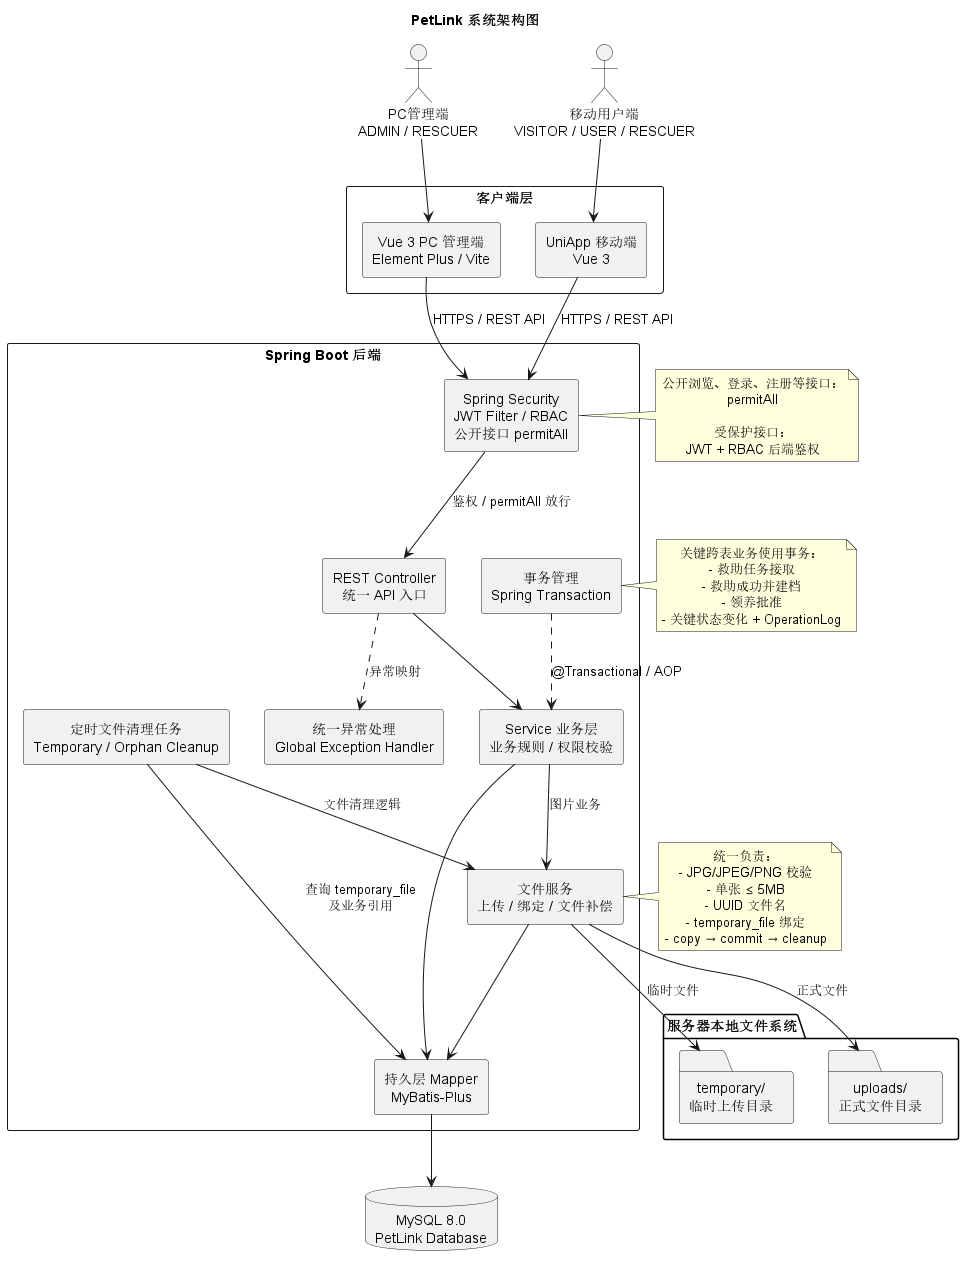
\includegraphics[width=0.92\textwidth]{system-architecture.png}
\caption{PetLink PC/Mobile 双端共享后端的系统架构}
\label{fig:architecture}
\end{figure}

\subsection{主体功能的完成状态}

本周合并和回归后，M01--M08 仍全部保持冻结完成状态。表~\ref{tab:modules} 按业务规则而非简单增删查改列出可验收成果。

\begin{longtable}{L{1.1cm}L{3.0cm}L{8.9cm}C{1.2cm}}
\caption{M01--M08 主体功能最终完成情况}\label{tab:modules}\\
\toprule
\rowcolor{PetGreen}\color{white}\bfseries 模块 & \color{white}\bfseries 业务范围 & \color{white}\bfseries 已完成成果 & \color{white}\bfseries 状态 \\
\midrule
\endfirsthead
\multicolumn{4}{l}{\zihao{5}\color{PetGray}表~\thetable\ （续）}\\
\toprule
\rowcolor{PetGreen}\color{white}\bfseries 模块 & \color{white}\bfseries 业务范围 & \color{white}\bfseries 已完成成果 & \color{white}\bfseries 状态 \\
\midrule
\endhead
\bottomrule
\endfoot
M01 & 用户与认证 & 注册、登录、JWT 鉴权、当前用户资料、账号状态与角色即时刷新；密码 BCrypt 存储、越权拦截与禁用会话均已测试。 & \pass \\
\rowcolor{PetPale}
M02 & 救助线索 & 普通用户提交带图线索，管理员审核通过或驳回；幂等键、请求指纹、文件绑定和操作日志已实现。 & \pass \\
M03 & 救助任务 & 待接取队列、原子接单、开始救助、过程记录和成功/失败收口；角色降级与活动任务的并发一致性已验证。 & \pass \\
\rowcolor{PetPale}
M04 & 动物档案 & 救助成功自动建档，包含多图、健康记录、性格观察、领养要求；支持治疗、观察、开放领养、暂停和恢复状态。 & \pass \\
M05 & 领养业务 & 申请、撤回、管理员审核、领养记录和同动物其他申请自动失效；审批事务按固定锁顺序执行。 & \pass \\
\rowcolor{PetPale}
M06 & 领养回访 & 回访提交、图片、历史查询和三角色可见性；永久幂等与并发重放恢复已完成。 & \pass \\
M07 & 收藏与公告 & 收藏/取消收藏幂等；公告草稿、编辑、发布、撤回、公开查看和带版本校验的逻辑删除已完成。 & \pass \\
\rowcolor{PetPale}
M08 & 管理与统计 & 用户禁用/启用、救助员角色生命周期、业务概览和趋势统计；敏感字段不进入列表响应。 & \pass \\
\end{longtable}

\section{新数据库合并与数据完整性}

\subsection{不直接覆盖的合并策略}

新数据库包与服务器正式库之间存在大量重复主键。如果简单导入或使用覆盖脚本，可能导致用户、线索、任务、动物和领养记录的关联关系错位。因此本次采用图~\ref{fig:db-flow} 所示的“隔离导入--映射合并--完整性验证”流程。

\begin{figure}[H]
\centering
\begin{tikzpicture}[
  node distance=1.05cm,
  box/.style={rounded corners=3pt,draw=PetGreen,line width=0.8pt,fill=PetPale,minimum width=10.8cm,minimum height=0.92cm,align=center},
  arrow/.style={-{Latex[length=2.5mm]},line width=0.8pt,draw=PetOrange}
]
\node[box] (a) {1. 备份正式库、部署文件和上传目录};
\node[box,below=of a] (b) {2. 将新数据库包导入隔离临时库};
\node[box,below=of b] (c) {3. 用户按 account 匹配，业务主键与外键统一重映射};
\node[box,below=of c] (d) {4. 在事务内按依赖顺序导入业务数据};
\node[box,below=of d] (e) {5. 检查外键孤儿、记录数与缺失的物理文件};
\node[box,below=of e] (f) {6. 提交事务，再生成部署后完整备份};
\draw[arrow] (a)--(b); \draw[arrow] (b)--(c); \draw[arrow] (c)--(d);
\draw[arrow] (d)--(e); \draw[arrow] (e)--(f);
\end{tikzpicture}
\caption{新数据库安全合并与验证流程}
\label{fig:db-flow}
\end{figure}

\subsection{数据合并成果}

合并脚本对每类业务记录建立新旧标识映射表，按用户、线索、任务、救助记录、动物、健康记录、领养申请、领养记录和操作日志的依赖顺序写入正式库。合并后的新增量和正式库最终数量见表~\ref{tab:db-counts}。

\begin{table}[H]
\centering
\caption{新数据库合并增量及正式库最终数量}
\label{tab:db-counts}
\rowcolors{2}{PetPale}{white}
\begin{tabularx}{0.88\textwidth}{Y C{3.2cm} C{3.2cm}}
\toprule
\rowcolor{PetGreen}\color{white}\bfseries 业务数据 & \color{white}\bfseries 本次新增 & \color{white}\bfseries 合并后总数 \\
\midrule
用户 & 11 & 24 \\
救助线索 & 13 & 26 \\
救助任务 & 6 & 13 \\
救助过程记录 & 1 & 5 \\
动物档案 & 6 & 10 \\
健康记录 & 4 & 8 \\
领养申请 & 4 & 7 \\
领养记录 & 1 & 3 \\
操作日志 & 66 & 168 \\
\bottomrule
\end{tabularx}
\end{table}

经检查，用户、线索、任务、动物、领养申请和领养记录的关键外键孤儿数均为 0。数据包中另有 16 条图片元数据找不到对应物理文件，本次主动不导入这些记录，避免页面出现破图。这一处理体现了“业务数据与文件必须同时存在”的完整性原则，而不是只追求导入行数。

\section{真实页面与 UI 成果}

\subsection{PC 公众首页与手机首页}

为确保报告中的界面与最终部署版一致，图~\ref{fig:dual-home} 为 2026 年 9 月 13 日从公网服务器实际页面获取的截图，不是原型图或静态设计稿。PC 端突出救助网络与公众参与入口，Mobile 端则将“我要领养”和“发布线索”放在拇指可及区域，两端保持统一品牌色彩和语义。

\begin{figure}[H]
\centering
\begin{subfigure}[t]{0.67\textwidth}
  \centering
  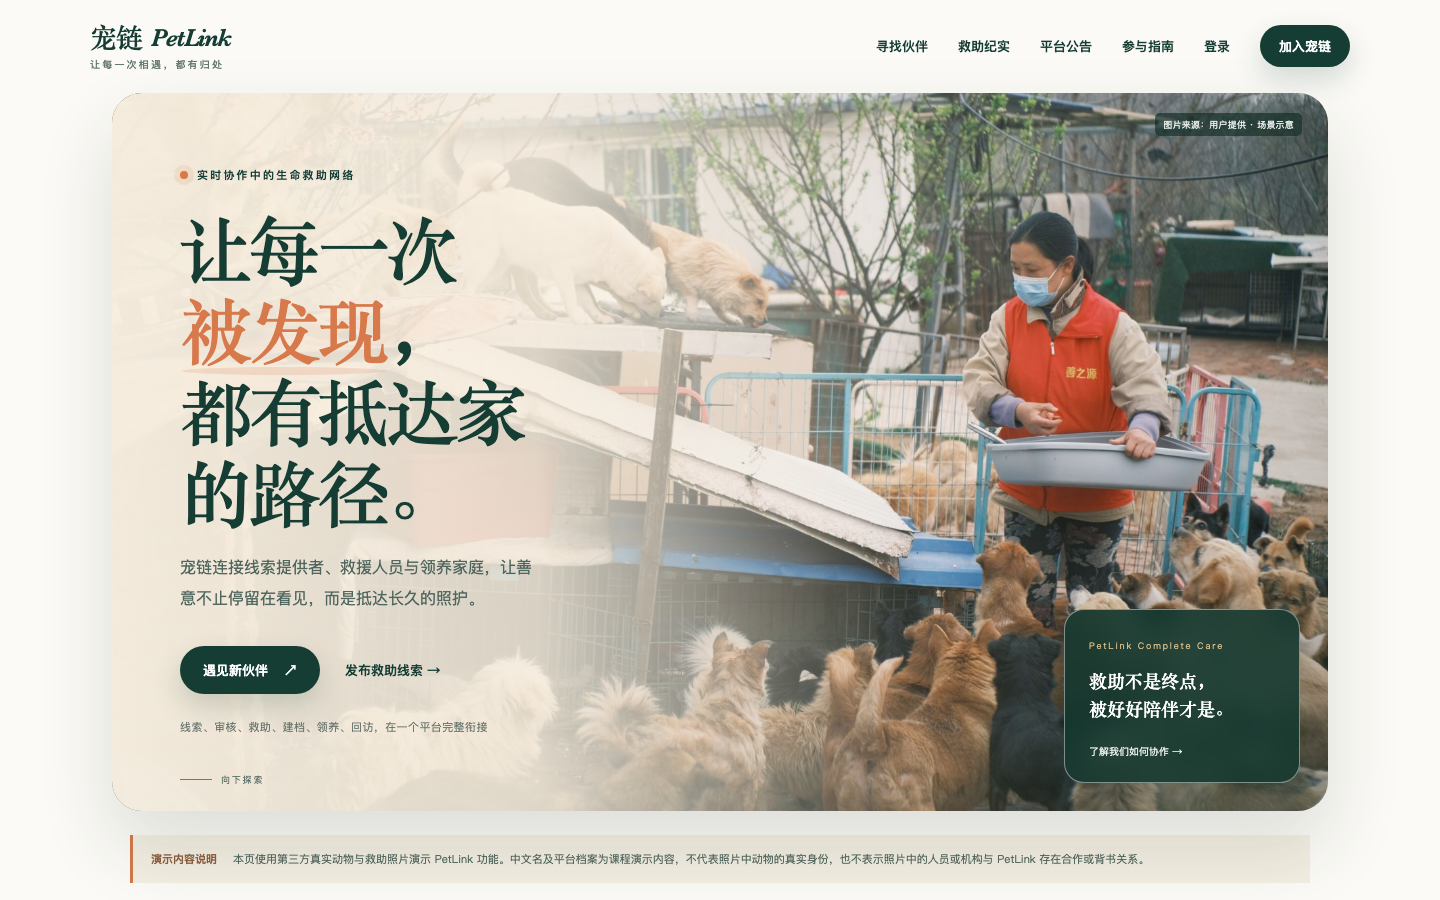
\includegraphics[width=\textwidth]{actual-pc-home-20260913.png}
  \caption{PC 端公众首页}
\end{subfigure}\hfill
\begin{subfigure}[t]{0.27\textwidth}
  \centering
  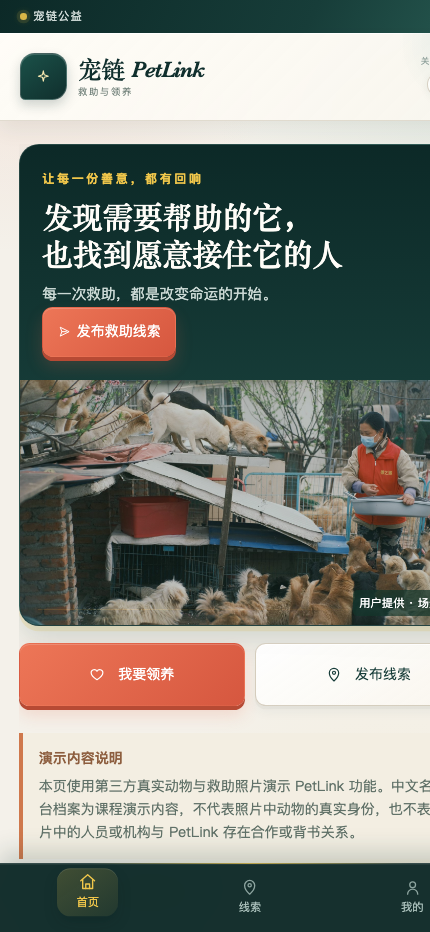
\includegraphics[width=\textwidth]{actual-mobile-home-20260913.png}
  \caption{Mobile H5 首页}
\end{subfigure}
\caption{公网部署版双端首页实际运行效果（2026-09-13）}
\label{fig:dual-home}
\end{figure}

\subsection{可领养动物列表}

图~\ref{fig:actual-adopt} 展示了正式数据库驱动的 PC 端可领养动物页面。页面已从原型阶段的固定卡片转换为 API 数据驱动，展示动物名称、物种、性别、年龄、健康摘要与当前状态。对于有图像的档案，前端通过受控媒体接口加载；如果图像不存在，统一回退到项目占位图，避免布局断裂。

\begin{figure}[H]
\centering
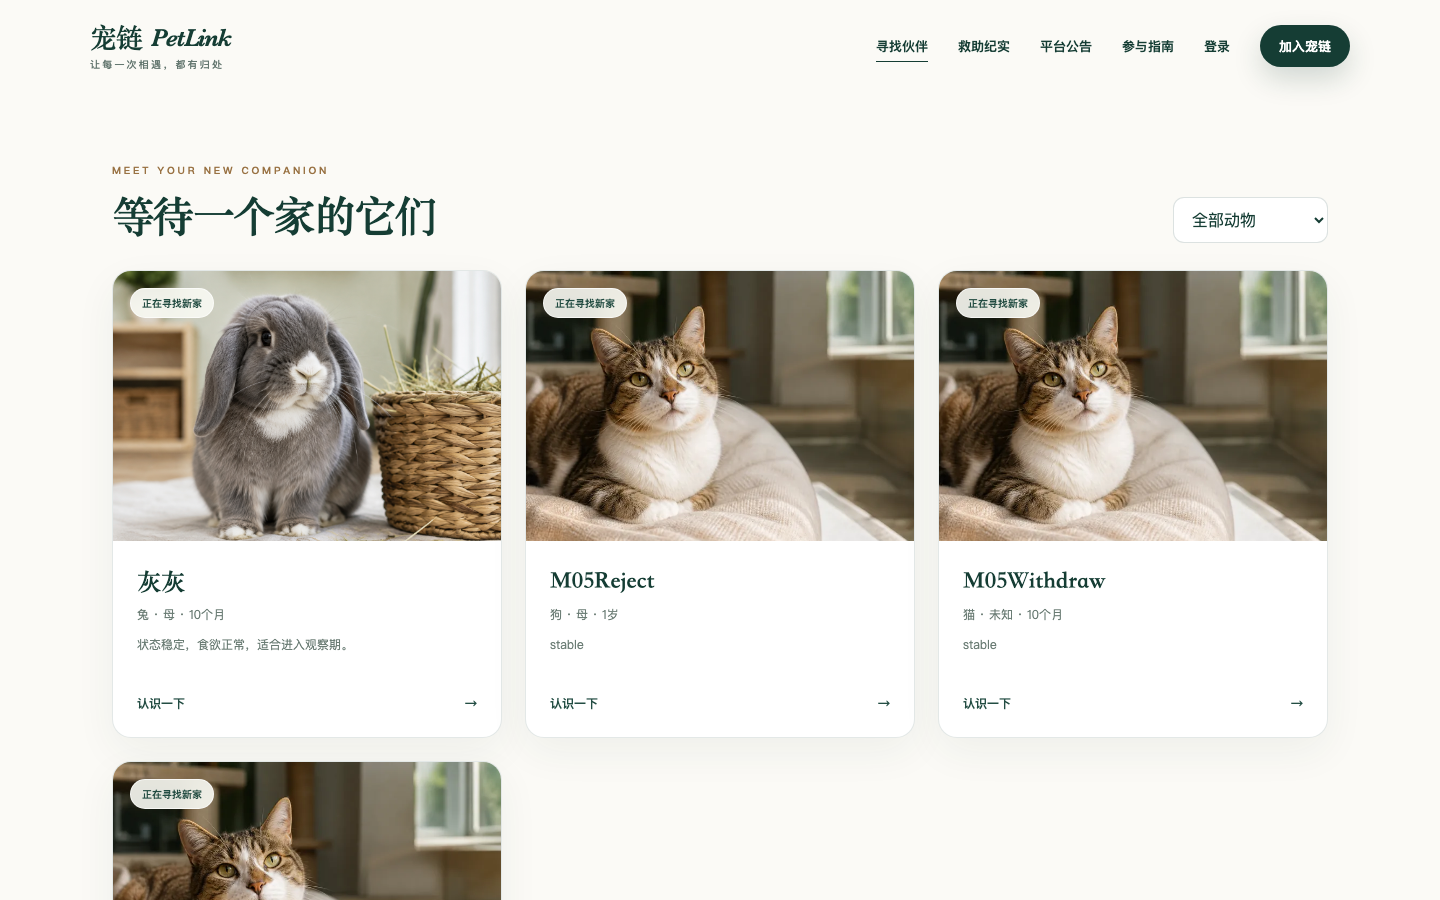
\includegraphics[width=0.95\textwidth]{actual-pc-adopt-20260913.png}
\caption{PC 端可领养动物列表实际页面（2026-09-13）}
\label{fig:actual-adopt}
\end{figure}

\subsection{救助纪实与完整档案表达}

本周新增的救助纪实页面如图~\ref{fig:actual-stories} 所示。每个演示档案不再只有“照片+名称”，而是将多张同一动物照片、健康情况、性格观察、领养要求和来源说明组织为结构化档案。页面还向下承载救助过程和领养回访，使产品内容与线索、任务、建档、领养、回访的业务链相互呼应。

\begin{figure}[H]
\centering
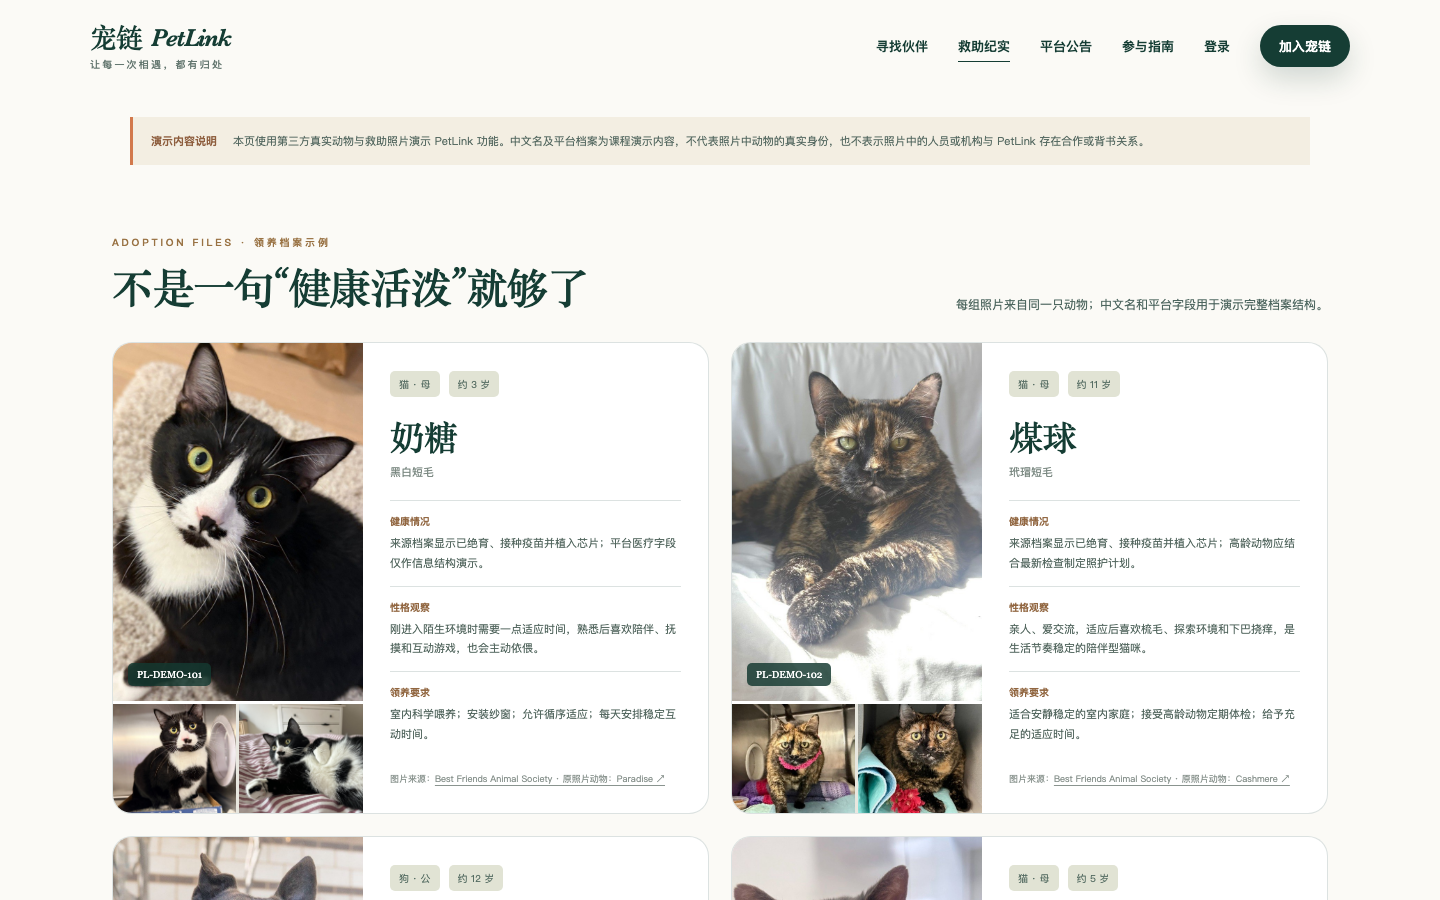
\includegraphics[width=0.95\textwidth]{actual-pc-stories-20260913.png}
\caption{PC 端救助纪实与完整动物档案实际页面（2026-09-13）}
\label{fig:actual-stories}
\end{figure}

上述截图均来自当前生产入口 \url{http://103.233.254.186:8081/}。页面中的公开案例均显示演示内容声明和图片来源；该内容用于展示 PetLink 的档案结构和 UI 能力，不将第三方公开案例表述为平台自有业务数据。

\section{测试完成情况与业务闭环}

\subsection{自动化门禁与生产构建}

合并后的后端使用 Eclipse Temurin JDK 17 环境重新执行 \code{clean test package}，所有 297 项 JUnit 测试通过后才生成生产 JAR。PC 与 Mobile 也分别执行全量 Node 测试和生产构建。各项结果见表~\ref{tab:test-gates}。

\begin{table}[H]
\centering
\caption{合并后自动化测试与构建门禁}
\label{tab:test-gates}
\rowcolors{2}{PetPale}{white}
\begin{tabularx}{\textwidth}{L{3.4cm}L{5.0cm}C{2.7cm}Y}
\toprule
\rowcolor{PetGreen}\color{white}\bfseries 子系统 & \color{white}\bfseries 验证方式 & \color{white}\bfseries 结果 & \color{white}\bfseries 判定 \\
\midrule
Spring Boot 后端 & JDK 17 / Maven 全量测试 & 297/297 & \pass\ 零失败、零错误 \\
PC 端 & Node 单元与组件测试 & 40/40 & \pass\ 包含新档案内容覆盖 \\
Mobile 端 & Node 单元与组件测试 & 21/21 & \pass\ 包含新字段与移动内容 \\
PC 构建 & Vite 生产构建 & 通过 & \pass\ 输出静态资源可部署 \\
Mobile 构建 & H5 生产构建 & 通过 & \pass\ 使用 \code{/mobile/} 基路径 \\
安全扫描 & 密码、JWT、环境文件入库检查 & 通过 & \pass\ 生产密钥不进入 Git \\
\bottomrule
\end{tabularx}
\end{table}

三个代码测试集共 358 项，全部通过。该数量不把生产 E2E 的 40 个步骤重复计入，以便区分“代码级自动化”和“部署环境业务验收”两类证据。

\subsection{双平台、三角色的40项线上 E2E}

本周最关键的测试成果是在公网部署环境中使用隔离验收账号执行一次完整业务流程，而不是仅依赖 Mock 或单个接口返回 200。流程如图~\ref{fig:e2e-flow} 所示，数据在 PC 与 Mobile 之间交替产生和消费，同时覆盖三类角色的权限边界。

\begin{figure}[H]
\centering
\begin{tikzpicture}[
  node distance=0.75cm and 0.38cm,
  flowbox/.style={rounded corners=3pt,draw=PetGreen,fill=PetPale,text width=2.55cm,minimum height=1.08cm,align=center,font=\scriptsize},
  arrow/.style={-{Latex[length=2.2mm]},draw=PetOrange,line width=0.8pt}
]
\node[flowbox] (s1) {USER / Mobile\\发布带图救助线索};
\node[flowbox,right=of s1] (s2) {ADMIN / PC\\查看并审核通过};
\node[flowbox,right=of s2] (s3) {RESCUER / 双端\\同步可见并接取};
\node[flowbox,right=of s3] (s4) {RESCUER / PC+Mobile\\开始救助并记录程};
\node[flowbox,right=of s4] (s5) {RESCUER / PC\\完成救助并建档};
\node[flowbox,below=of s1] (s6) {USER / Mobile\\收藏并提交领养申请};
\node[flowbox,right=of s6] (s7) {ADMIN / PC\\审批并生成领养记录};
\node[flowbox,right=of s7] (s8) {USER / Mobile\\提交幂等领养回访};
\node[flowbox,right=of s8] (s9) {RESCUER / PC\\查看所负责动物回访};
\node[flowbox,right=of s9] (s10) {ADMIN / PC\\发布公告并核对统计};
\draw[arrow] (s1)--(s2); \draw[arrow] (s2)--(s3); \draw[arrow] (s3)--(s4); \draw[arrow] (s4)--(s5);
\draw[arrow] (s5.south) -- ++(0,-0.28) -| (s6.north);
\draw[arrow] (s6)--(s7); \draw[arrow] (s7)--(s8); \draw[arrow] (s8)--(s9); \draw[arrow] (s9)--(s10);
\end{tikzpicture}
\caption{PC/Mobile 双平台与三角色线上业务闭环}
\label{fig:e2e-flow}
\end{figure}

40 个验收步骤可归纳为表~\ref{tab:e2e-groups} 中的八组业务能力。其中特别针对先前易出问题的“审核通过后救助人员看不到待接取任务”进行了双端同时断言：线索进入 \code{WAITING\_ACCEPT} 后，PC 和 Mobile 的救助人员列表均能找到同一条记录；接取成功后，该记录又会同步移出待接取列表。

\begin{table}[H]
\centering
\caption{部署后 40 项 E2E 验收覆盖}
\label{tab:e2e-groups}
\rowcolors{2}{PetPale}{white}
\begin{tabularx}{\textwidth}{L{3.6cm}Y C{2.1cm}}
\toprule
\rowcolor{PetGreen}\color{white}\bfseries 验收组 & \color{white}\bfseries 核心检查 & \color{white}\bfseries 结果 \\
\midrule
环境与登录 & 健康检查、Mobile Origin/CORS、三角色登录与跨端令牌 & \pass\ 通过 \\
线索与幂等 & 图片上传、幂等键、Mobile 发布、PC 重放与审核 & \pass\ 通过 \\
待接取双端同步 & 审核通过后 PC/Mobile 同时可见，接取后同步移除 & \pass\ 通过 \\
救助任务与建档 & 开始、过程记录、成功收口、线索关闭、完整动物字段 & \pass\ 通过 \\
动物状态机 & 治疗中转观察中，再开放领养，普通用户可见且隐藏内部标识 & \pass\ 通过 \\
领养与回访 & 收藏跨端同步、申请、审批、领养记录、回访幂等与救助员可见 & \pass\ 通过 \\
公告与统计 & PC 创建并发布公告，Mobile 可见，统计返回 7 类业务组 & \pass\ 通过 \\
账号与权限隔离 & 禁用/恢复立即生效，USER 不能访问 ADMIN 或 RESCUER 专属接口 & \pass\ 通过 \\
\bottomrule
\end{tabularx}
\end{table}

验收过程中的临时账号、线索、动物、公告和图片全部带唯一批次标记；测试通过后按明确主键定向清理，未删除原有业务数据，也没有把“验收公告”等内容留在公开页面。

\section{服务器发布、备份与回滚准备}

\subsection{生产发布结果}

最终版本已部署到 Ubuntu 22.04 服务器，由 Docker Compose 管理 MySQL、Spring Boot 后端和 Nginx Web 三个服务。PetLink 使用 8081 端口，服务器原有 80 端口项目未受影响。更新过程只重建后端与 Web 容器，没有删除或重建 MySQL 数据卷，也没有覆盖上传文件目录。

\begin{table}[H]
\centering
\caption{生产环境运行与访问状态}
\label{tab:deployment}
\rowcolors{2}{PetPale}{white}
\begin{tabularx}{\textwidth}{L{3.4cm}Y C{2.5cm}}
\toprule
\rowcolor{PetGreen}\color{white}\bfseries 验证对象 & \color{white}\bfseries 实际地址/状态 & \color{white}\bfseries 结果 \\
\midrule
PC 公众站 & \url{http://103.233.254.186:8081/} & HTTP 200 \\
救助纪实 & \url{http://103.233.254.186:8081/stories} & HTTP 200 \\
Mobile H5 & \url{http://103.233.254.186:8081/mobile/} & HTTP 200 \\
健康检查 & \url{http://103.233.254.186:8081/health} & \code{UP} \\
原有服务 & \url{http://103.233.254.186/} & HTTP 200 \\
Docker 容器 & backend、web 运行，mysql 健康 & \pass\ 正常 \\
\bottomrule
\end{tabularx}
\end{table}

\subsection{可回滚的发布过程}

发布前已保存正式数据库、部署文件、上传文件和环境配置的完整备份；原后端与 Web 镜像已标记为 \code{rollback-20260912-pre-merge}。部署后完成全部验收并清理临时数据，又生成一份最终干净备份。两个备份节点见表~\ref{tab:backups}。

\begin{table}[H]
\centering
\caption{合并部署的关键备份与回滚证据}
\label{tab:backups}
\rowcolors{2}{PetPale}{white}
\begin{tabularx}{\textwidth}{L{3.3cm}Y L{3.0cm}}
\toprule
\rowcolor{PetGreen}\color{white}\bfseries 节点 & \color{white}\bfseries 备份位置 & \color{white}\bfseries 用途 \\
\midrule
合并前 & \path{/srv/petlink-backups/20260912-123418-pre-merge} & 快速恢复原正式数据与部署文件 \\
合并部署后 & \path{/srv/petlink-backups/20260912-215754-post-merge-final} & 保存已验收、已清理的最终上线基线 \\
容器镜像 & \code{rollback-20260912-pre-merge} & 在应用层快速回退后端和 Web 版本 \\
\bottomrule
\end{tabularx}
\end{table}

备份文件已生成 SHA-256 校验清单，可在恢复前检查传输完整性。此外，合并脚本在仓库中默认以 \code{ROLLBACK} 结尾，只有在隔离环境演练和数量校验通过后，才在服务器执行副本中显式改为 \code{COMMIT}，从脚本默认值上降低误操作风险。

\section{代码归档、交付物与质量证据}

本周代码和说明材料已提交到 Git 主分支并推送到 GitHub。最终服务器部署版与仓库主分支保持一致，工作区无未提交文件。主要变更和证据见表~\ref{tab:deliverables}。

\begin{table}[H]
\centering
\caption{第2周主要代码与质量交付物}
\label{tab:deliverables}
\rowcolors{2}{PetPale}{white}
\begin{tabularx}{\textwidth}{L{3.3cm}Y L{3.2cm}}
\toprule
\rowcolor{PetGreen}\color{white}\bfseries 交付物 & \color{white}\bfseries 内容 & \color{white}\bfseries 位置/标识 \\
\midrule
产品内容与档案合并 & 动物完整档案、救助纪实、双端内容图片和扩展测试 & Git \code{02a53e5} \\
数据库合并脚本 & 主键/外键重映射、导入数量统计和缺失文件排除 & 数据合并 SQL \\
跨平台 E2E 脚本 & 支持独立健康检查地址，断言新动物字段的真实传递 & E2E JavaScript \\
部署验收记录 & 合并数量、测试结果、运行状态、备份与回滚说明 & 部署合并验收文档 \\
最终验收提交 & 文档、合并脚本和验收脚本推送主分支 & Git \code{83964ba} \\
\bottomrule
\end{tabularx}
\end{table}

本次归档不包含真实服务器 \code{.env}、数据库密码、JWT 密钥、用户明文密码或上传数据，这些内容只在部署环境中管理。公开仓库仅保留环境变量示例、带默认回滚保护的数据合并脚本和不包含凭据的验收记录。

\section{是否完成全部开发和测试}

\subsection{开发完成性判定}

从详细设计说明书与 M01--M08 冻结基线看，项目已完成全部计划内主体功能，不存在未实现的核心业务模块。本周合并的新字段和内容页面已通过代码级测试和线上 E2E，没有破坏原 72 个 Frozen REST 路由、方法、鉴权或状态机约定。

\subsection{测试完成性判定}

后端、PC、Mobile 的全量自动化门禁全部通过，生产构建成功，双平台三角色的 40 项业务闭环也已在公网环境中通过。因此，可以判定“计划内自动化和核心业务测试已完成”。仍需的浏览器和真机人工抽查是为了提升课程交付稳定性，并不代表当前存在已知核心功能缺陷。

\subsection{余下 2\% 的工作与时间估算}

\begin{table}[H]
\centering
\caption{交付前余下工作与预计时间}
\label{tab:remaining}
\rowcolors{2}{PetPale}{white}
\begin{tabularx}{\textwidth}{L{4.2cm}Y C{2.2cm}}
\toprule
\rowcolor{PetGreen}\color{white}\bfseries 余下工作 & \color{white}\bfseries 完成标准 & \color{white}\bfseries 预计用时 \\
\midrule
Chrome/Edge 关键页面人工抽查 & 登录、待接取、动物档案和领养审核无布局与交互阻塞 & 0.5 天 \\
HBuilderX 与 Android/iOS 真机复核 & 核心表单、图片选择、底部导航和移动端登录可用 & 0.5--1 天 \\
最终回归和证据归档 & 固定提交版本，核对备份、测试报告、截图与项目文档相互一致 & 0.5 天 \\
非阻塞体验优化 & 仅处理复核中发现的文案、间距或小屏适配问题 & 0--0.5 天 \\
\midrule
\textbf{总计} & \textbf{不新增功能范围，完成课程交付收尾} & \textbf{1--2 天} \\
\bottomrule
\end{tabularx}
\end{table}

预计在 2026 年 9 月 14--15 日完成上述余量。即使人工复核发现非阻塞小问题，因为代码基线、全量自动化、生产环境和回滚机制均已具备，项目组有能力在 1--2 天内完成修正与再验证。

\section{阶段总结}

第三阶段第2周的核心成果不是单纯增加页面数量，而是完成了一次面向真实交付的集成与验证：新版源码被有选择地合入冻结基线，存在主键冲突的新数据库通过映射事务安全合并，缺失物理文件的图片元数据被明确排除，合并后版本在 JDK 17 中通过全量后端测试，并在公网环境中完成 PC/Mobile 两端、USER/RESCUER/ADMIN 三角色的完整业务闭环。

因此，项目组对当前进度的最终判定为：\textbf{总体进度 98\%，主体开发和核心测试基本全部完成，项目已具备稳定演示、继续回归、数据备份和快速回滚能力。}余下工作不扩大功能边界，仅用于独立环境人工复核与课程交付收尾，预计再需 1--2 天。

\end{document}
